
\section{Research Contributions \& Implications}

The overarching goal of this dissertation was to analyze trends of growing rates of poverty in the suburbs of Canadian cities during the late 20th and early 21st centuries; and how this affects daily travel, activity participation, and social inclusion. Chapter \ref{ch:background} provided a background and discussion of previous research on the related issues. This was followed by three innovative empirical analyses (Chapters \ref{ch:subtrapov}, \ref{ch:pathsubpov}, \ref{ch:lowinctra}), each of which developed important contributions to theoretical and empirical knowledge on these issues.

% problem
Chapter \ref{ch:subtrapov} was motivated by how a potential negative impact of suburbanization of poverty is that lower-income households are re-locating to areas that are more auto-oriented, less walkable, and have relatively lower levels of public transit service than central areas. This could be resulting in longer commutes and increased barriers to daily activity participation, especially for those who are unable to afford a private vehicle. The ability to travel to important activity destinations is vital for economic independence (e.g. finding and retaining employment), health, and well-being - and at a greater scale, it can contribute to robust urban economies and healthier societies as a whole. In the worst cases, dissuasion or inability to travel to important destinations can limit activity participation, result in social exclusion, and negatively impact the vitality of urban environments \cite{lucas_transport_2012,martens_transport_2016}. However, previous research on suburbanization has not considered it's relation to transportation and travel behaviour beyond brief discussion that it is a potential impact \shortcite<e.g.>{hulchanski_three_2010,walks_social_2001,ades_are_2012,breau_pulling_2018, grant_changing_2020}. 

Accordingly, this chapter combines data sources to analyze the relationships between increasing socio-spatial inequalities (e.g. de-centralization of low-income households), transport disadvantage (e.g. spatial distribution of zero-car households, low levels of transit accessibility), and adverse travel behaviour outcomes (e.g. lengthier commute times and lower activity participation rates). Using methods include computing transit accessibility metrics that are comparable over time, statistical mapping, modelling changes in travel behaviour over time, and visualizing neighbourhood change with respect to levels of suburbanization. In particular, the spatio-temporal neighbourhood modelling is a quantitative strategy that has not been used in neighbourhood studies in Canada. So while focused on Toronto, these methods can certainly be transferable to other regions where there is available data.

In terms of findings, this study provides solid evidence that transport poverty in Toronto is increasing more in the suburbs relative to central areas. Eastern suburbs in particular have suffered the most, indicative by having the greatest combination of increased transport and social disadvantage, and evidenced by increasing commute times and declining daily activity participation rates. Our research thus confirms theoretical pathways of transport poverty \cite{lucas_transport_2012}, and moreover, shows that it is occurring more within suburban neighbourhoods.

% then lead into next, highlight importance of individual
However, this Chapter (\ref{ch:subtrapov}), like most previous studies analyzing suburbanization of poverty and neighbourhood change more generally \cite{ades_are_2012,breau_pulling_2018,grant_changing_2020} were based on neighbourhoods. But neighbourhood-level analysis could be masking individual effects since we only analyzed change at a neighborhood level. For example, there could be more extreme levels of travel be outcomes in later years than earlier years in certain neighborhoods. Nor is it known whether upward or downward socio-economic status in a neighbourhood is primarily due to residential mobility or residents becoming poorer or wealthier in-place.

As such, the next two Chapters (\ref{ch:pathsubpov} and \ref{ch:lowinctra}) make use of individual-level panel data, specifically the Longitudinal Admininstrative Databank (LAD), a panel dataset of annual tax filers, to examine intra-urban moves relative to transportation and urban form.

Chapter \ref{ch:pathsubpov} is particularly motivated by how ample research (includuing Chapter \ref{ch:subtrapov}) has described trends of suburbanization of poverty at regional and neighbourhood levels, but has been unable to discern how residents end up to become poor and living in the suburbs. This Chapter first develops a conceptual framework describing different potential pathways to suburban poverty, and then uses the LAD to quantify these pathways across urban regions in Canada. This analysis specifically estimates for the first time in Canada to what extent suburban poverty stems from intra-urban residential mobility, external immigration, and remaining poor in-place---thus providing an important link between theory and empirical evidence on the urban dynamics that lead to suburbanization of poverty. Understanding the propensity of these pathways provides important knowledge regarding the urban dynamics that lead to contemporary suburban geographies of poverty concentration. Such knowledge can also be helpful for planning and policy including (but not limited to) public transit prioritization, providing resources for recent immigrants, protections against displacement, and social housing policy; and overall, aiming to reduce the burdens of being poor and living in the suburbs.

This analysis shows that suburban poverty is an increasing phenomenon in Canadian cities. This is evident in our analysis of tax records (see Figure \ref{fig:subpov4}) as well as previous research using census and other survey data \cite{ades_are_2012,breau_pulling_2018,grant_changing_2020,allen_suburbanization_2021}. Importantly, the data indicate that transitioning to suburban poverty on an annual basis is much more a result from staying or becoming poor within the suburbs compared to immigration or due to moving (and potentially being displaced from) gentrifying neighbourhoods in the centre. On a year-by-year basis, of the low-income suburban residents who lived in the suburbs, 21.5\% dropped into poverty while staying in the suburbs on average, compared to only 2.9\% who moved from a central area or the 6.6\% who immigrated from elsewhere. We find that these trends are similar when comparing between regions and over our study period (2006 to 2016). Despite this finding, much of the discussion in Canada on suburbanization of poverty has been directly attributed to gentrification and displacement from less affordable central neighbourhoods \cite{grant_changing_2020}. This points to further consideration into the causes of dropping into poverty in the suburbs including (but not limited to), increasing rents in suburban apartments \cite{august_gentrification_2018}, automobile debt limiting spending in other areas \cite{walks_driving_2018}, or low transit accessibility impacting ability to travel to employment, education, or social services needed for poverty reduction \cite{allen_planning_2020} 

Chapter \ref{ch:lowinctra} directly looked at whether there is evidence of a disproportionate number of low-income residents moving away from relied upon public transit service, and if so, how this has changed over time. Specifically, it measured changes in transit accessibility experienced by intra-urban movers by income level. Findings show that low-income residents, on average, decrease their transit accessibility when they move. This has important social inclusion implications since many low-income residents are reliant on public transit for travelling to daily activities \cite{allen_planning_2020,barri_can_2021}, including finding employment \cite{fransen_relationship_2019,bastiaanssen_does_2021}. Moving away from relied upon public transit could thus decrease capabilities for activity participation, and in some cases, increase risks of transport-related social exclusion \cite{lucas_transport_2012,allen_planning_2020}.

Importantly, we also find that low-income residents do not decrease their transit accessibility when moving at a greater rate than non-low-income residents. This is despite ample neighbourhood-level research describing inner-city gentrification occurring in Toronto over the past several decades \cite{hulchanski_three_2010,walks_gentrification_2021}. In fact, we find that non-low-income residents living in central areas are more likely to move out of these neighbourhoods than compared to low-income residents, and on average experience greater reductions in their levels of transit accessibility when they move. This difference in findings is likely because the unit of analysis of our study were individuals rather than neighbourhoods, meaning that gentrification observed at a neighbourhood level is likely partly due to upward income mobility of residents who stay in these neighbourhoods or affluent residents moving in from outside the study region (either national or international immigrants). As well, we also find that much of the outward residential mobility by non-low-income households noted in 20th century urban theory \cite{burgess_growth_1925,alonso_location_1964} has continued to persist in Toronto. In particular, the outer suburbs and exurbs of Toronto are predominately exclusive to non-low-income residents compared to other areas. While our empirical analysis was focused on Toronto, the data and methods described in this chapter provide a template which could be applied elsewhere. 

Even though we find that low-income residents are not disproportionately moving away from transit relative to non-low-income residents, gentrification and increasing costs of housing are still likely leading to changing spatial patterns of low-income neighbourhoods in the region. In Toronto, the most affordable housing is located in the inner-suburbs as mid-20th century apartment towers \cite{skaburskis_filtering_2014,august_gentrification_2018}. The formation of low-income neighbourhoods in these inner-suburban neighbourhoods, but without evidence of substantial displacement and residential exclusion in central neighbourhoods, indicates that these observed increases in suburbanization of poverty in Toronto is more likely due to immigrants with lower incomes settling in the suburbs or residents becoming and remaining poor in-place within the suburbs (this aligns with findings from Chapter \ref{ch:pathsubpov})

%Overall, in conjunction, these three quantitative analyses QQQQQ
%Furthermore, findings about differences in individual residential mobility patterns by income and relative to transit accessibility can offer further explanations about how contemporary trends of urban socio-spatial restructuring, such as inner-city gentrification and suburbanization of poverty, unfold within a region over time. 


% Specifically, we use a combination of census and transportation network data to create a typology of suburbanization via a hierarchical $k$-means cluster analysis. We then link this typology to panel data representing 20\% of tax filers across Canada to examine immigrant settlement patterns and residential mobility trajectories of low-income households, grouped by typologies of suburbanization. 




% Specifically, for those in suburban poverty in Canadian CMAs, 88.5\% lived in the suburbs a year prior (of which, 12.7\% moved residences within the suburbs and 75.8\% did not move), 2.9\% moved from a central neighbourhood, and 6.6\% immigrated from elsewhere (4.6\% internationally, 2.0\% from within in Canada). Moreover, of the low-income suburban residents who lived in the suburbs a year prior, 21.5\% were not classified as being in a low-income in the previous year. Thus becoming poor while staying in the suburbs encompasses a greater proportion of suburban poverty than immigration and \textit{centre}-to-\textit{suburb} mobility combined. 



Overall, our results provide pertinent information to aid preventative policy aimed at reducing suburban poverty in Canada. For one, knowledge that a substantial portion suburban poverty stems from becoming poor in-place should expedite support for urban planning and policy to make suburbs more livable and accessible. In other words, policy for reducing suburban poverty should not parochially be focused on other pathways, such as limiting gentrification and displacement. While important to quell such displacement, our findings indicate that it is also imperative to make improvements to the suburbs, such as expanding community and social resources in the suburbs alongside more compact urban design, active travel infrastructure, and improved public transit in order to provide residents the ability to access amenities and opportunities (e.g. employment, education), as these would all be worthwhile strategies aimed at poverty alleviation in the suburbs. These are not new ideas. Many of them have been advocated for previously in terms of reducing the negative population health and environmental impacts associated with auto-oriented environments \shortcite{cervero_travel_1997,ewing_relationship_2003,ewing_compactness_2015}, and limiting the detrimental impacts suburbanization of poverty has on increasing polarization and segregation of urban space as well as the negative impacts caused by eviction and displacement on individual well-being and community cohesion  \shortcite{hulchanski_three_2010,ades_are_2012,walks_income_2013,august_challenging_2014,august_its_2016}. Findings additionally show that international immigrants have a high propensity of settling in the suburbs and being below the poverty line. This points to policy aimed at providing incentives for more housing (e.g. as vouchers) for recent immigrants, particularly in more central locations.


% Our findings additionally show that international immigrants have a high propensity of settling in the suburbs and being below the poverty line. This points to policy aimed at providing incentives for more housing (e.g. as vouchers) for recent immigrants, particularly in more central locations. 

% Policy to reduce these effects should thus have a two-pronged approach. The first is to curb the growth of suburban poverty through focusing on increasing the supply of affordable housing in areas with high transit accessibility, having strong rent controls, and preventing forced eviction and displacement from central to suburban neighborhoods. The second is to upgrade suburban environments through transport planning and urban design strategies that improve transit accessibility and walkability (i.e. improving accessibility at both neighborhood and regional scales). 





\section{Data Limitations}

This dissertation has several limitations that stemmed from a lack of data.

First off, historical analysis transport (dis)advantage in Chapters \ref{ch:subtrapov} and \ref{ch:lowinctra} were mainly assessed in terms of transit access to destinations and auto ownership. This did thus not consider other components of urban form that could either benefit or detriment urban living \cite{ewing_relationship_2003,ewing2014measuring}. Suburban built environments typically remain focused on the car, which have a number of safety and environmental concerns (e.g. speed limits are greater, safe crossings are more spread out, creating barriers to active travel). On the other hand, some suburban areas offer better access to green space, which can have a positive effect on health and well-being. Future research should consider other positive and negative environmental impacts of less-centralized urban living for low-SES populations. This could prove challenging, however, since there is little readily available historic data on urban form, walkability, and access to green space. This lack of data was the main reason research in these chapters only looked at transit accessibility.

The accessibility measures used in \ref{ch:subtrapov} and \ref{ch:lowinctra} as well as the historical travel behaviour (activity participation and commute times) used in \ref{ch:pathsubpov} were reliant on as travel survey that represented only a 5\% sample of the population, limiting analysis at smaller geographic scales. Secondly, there may have been some inconsistencies with how data were collected across survey years. Variables were selected that were consistently defined over time based on survey documentation, but there were likely some imperfections in interpretation and administration of survey questions. Prior to 2016, the travel survey did not ask respondents about income, limiting any historical analysis on jobs accessible by low-income status. Such data would be arguably a better measure for measuring accessibility for low-income residents \cite{fan_impact_2012,cui_accessibility_2019,allen_sizing_2019}. As well, in terms of data historical travel survey and census data, there was likely some inaccuracy caused by the data harmonization process of apportioning data to the same spatial units over time. These issues are unavoidable when dealing with longitudinal survey data that has been aggregated to different areal units \cite{allen_new_2018}. 

The multi-city analysis in Chapter \ref{ch:pathsubpov} only focused on year-to-year transitions from 2006 to 2016. An important direction for future work would be to analyze individual pathways to suburban poverty prior to 2006, however this was limited due to the lack of historical transit accessibility measures in other regions. If this data existing, it would allow for extending Chapter \ref{ch:pathsubpov} and \ref{ch:lowinctra} to incorporate comparative analyses across multiple cities to assess whether there are consistencies or differences in findings regarding whether low-income residents are unequally moving away from transit.

Chapter \ref{ch:pathsubpov} and \ref{ch:lowinctra} both used the Longitudinal Administrative Databank (LAD) to examine residential moboility by poverty status. One drawback of using this tax record data (the LAD) is that it lacks contextual factors about why people move. Such factors are difficult to directly infer from tax records, for instance, whether moves are due to preferences or constraints, and what the main push or pull factors are. The LAD inclcudes a single binary measure of low-income status (LIM), which was used to classify whether a resident was in poverty in a given year. This was used out of convience, because it was pre-defined by Statistics Canada as well as used in other research projects \cite{picot_immigration_2014,allen_sizing_2019,brown_money_2019}. However, sensitivity analysis of results for different poverty measures, including those with multiple categories, would allow for more nuanced findings. 

Similarly, Chapter \ref{ch:pathsubpov} includes generating a binary measure via a cluster analysis to describe whether or not a neighbourhood is suburban. This could be expanded to looking at multiple categories of urban form, in particular, specific types of suburban neighbourhoods. The $k$-means hierarchical clustering method we used could certainly be expanded to account for this. As well, other clustering methods could be tested to examine how and to what extent they would affect results.

% develops a conceptual framework and empirically examines residential mobility pathways to suburban poverty. But given the exploratory nature of this analysis, as well as use of a large-sample dataset, some simplifications were made. 

These problems also highlight the need in the future for individual-level linked datasets, similarly to how medical records have been linked to census data in health research. Analyzing individual panel data would be helpful for examining pathways to suburban poverty and whether improvements in transit accessibility are either more likely to alleviate poverty or result in gentrification and displacement. For example, linking individual census data longitudinally, to travel survey data, to tax records, to surveys like the General Social Survey, would open up an abundance of research possibilities. While there would be privacy concerns, such linkages should be possible for researchers at Research Data Centres.



\section{Future Research}

Beyond improving data collection and efforts, this research leads to several directions for additional theoretical, methodological, and empirical research. 

As noted earlier, the findings of this dissertation have several implications for urban planning and policy, particularly regarding transportation and housing. However, this dissertation did not look directly at the effectiveness of any particular project or policy intervention. As such, future research could be designed to study the effectiveness of different strategies of reducing the propensity of dropping into poverty in the suburbs. This could include examining the effects of infrastructure (e.g. new or improved public transit infrastructure, cycling infrastructure, pedestrian improvements) or broader land-use policies (e.g. intensification, implementation of 15-minute cities) on various social and travel behaviour outcomes analyzed in this dissertation (e.g. activity participation, commute times, residential mobility) as well as others (e.g. income mobility, mode share, etc.).

% transit induced displacaement:
For example, expanding upon Chapter \ref{ch:lowinctra}, future analysis could look at the residential mobility results of new transit infrastructure. 

Similar research has been conducted in the United States with mixed findings \cite{delmelle_new_2020, delmelle_transit-induced_2021}

 Another direction for future work could be to link this data to possible push or pull factors that may disproportionately affect residential mobility of low-income residents. For example research analyzing out-mobility due to gentrification and new transit infrastructure has been conducted in the United States \cite{freeman_displacement_2005,delmelle_new_2020}, but not in Canada, and nowhere that we are aware of with the sample size of the LAD (20\% of the population). Continuing research in these directions would provide further knowledge regarding the individual pathways and neighbourhood dynamics that lead to suburbanization of poverty.

% 







Ample research has shown that compact urban forms and greater levels of transit accessibility promote more environmentally friendly outcomes and healthier lifestyles \cite{ewing_compactness_2015,ewing_travel_2010,cervero_travel_1997}. There are also theoretical arguments that accessibility is a social good, as it enables activity participation \cite{martens_transport_2016,pereira_distributive_2017}. But what about long-term benefits? Can such built environments also lead to social mobility and poverty reduction? Research has noted how neighbourhood socio-economic effects impact individual social mobility \cite{chetty_effects_2016}, yet research on how urban form, and in particular transit accessibility has on long term social outcomes is sparse \cite{ewing_does_2016,fransen_relationship_2019}. Findings in Chapter \ref{ch:pathsubpov} indicate that a substantial amount of residents drop into poverty in the suburbs, but this research was not directly asking why and how this is related to urban form. As such, future research could use similar data in this dissertation to uncover whether low-income residents exposed to more compact urban forms and better levels of transit accessibility have relatively greater income mobility over time relative to areas of worse accessibility, while controlling for other demographic and stage-of-life effects, as well as residential mobility and exposure to different urban forms. However, since the LAD and census do not have variables on car ownership (an important predictor of employment), such data would have joined to other survey or administrative data.

as well as analyze individuals over the course of multiple years. The latter could be conducted via sequence analysis methods to examine whether there are common life-course and residential mobility trajectories to suburban poverty. This could also be used to connect to longer-term neighborhood-level changes (e.g. to ask whether neighbourhoods with more concentrated poverty have a larger share of low-income people who dropped into poverty or who moved from elsewhere?). 

This dissertation, and the aforementioned directions for future work, are retrospective. It is clear though that cities are dynamics, and that urban futures are rife with uncertainty. Yet when planners and researchers assess the distributions of transit accessibility benefits across different socio-economic groups, they are typically based on current distributions. However, the demographic patterns of cities change over time, as recently evidenced by socio-spatial polarization, gentrification, and suburbanization of poverty \cite{ades_are_2012,van_ham_understanding_2013,grant_changing_2020}, additionally shown by the findings in this dissertation. As such, transport planners should be mindful of potential socio-economic changes when they examine current and future distributions of transport accessibility, as they can directly relate to social (in)equity and transport-related social exclusion. Accordingly, future research should explore how the distributions of transit accessibility relative to socio-econmoic status can vary substantially depending on different future socio-economic trajectories. Examples of differing trajectories include gentrification versus affordable near transit and polarization versus evenness. 

This could be explored through a theoretical discussion and conceptual examples; simulating data based on current population, employment, and transit travel time data as base, and apply ranges of outcomes based on the above dimensions. Simulations could make use of Markov chain Monte Carlo methods, based on stochastic transition matrices generated by parameters relating to polarization-evenness, gentrification-affordability, homophily, and spatial focus of residential mobility. These issues could also be explored via using a regional travel demand model (such as the one used in the Toronto region), tweaking it's residential mobility sub-model.  In other words, it will provide differing outputs for population, land-use, and travel times depending on variation in input parameters. This will allow for computing accessibility measures for multiple scenarios, rather than comparing multiple socio-economic distributions with a single accessibility distribution. My current expectation is that results will likely indicate that compact urban forms, focused on affordable housing near transit will reap the greatest benefits in terms of social equity and social inclusion.

Future research could also focus on developing more theoretical or conceptual frameworks on neighbourhood change and neighbourhood effects, particularly as they relate to transport and land use. Neighbourhoods are the stage for daily life. Individuals' neighbourhood contexts can impact a number of social outcomes; from daily travel behaviour and activity participation, to longer-term effects on employment, income, health, and well-being \cite{sampson_assessing_2002,ewing_travel_2010,lucas_transport_2012,bastiaanssen_does_2020}. However, environmental contexts change over longer period of time, both in terms of their built environments (e.g. due to land use intensification, transit (dis)investments) and social attributes (e.g. socioeconomic decline, gentrification) \cite{van_ham_understanding_2013,wegener_land-use_2004}. Therefore, one's environmental exposures are not static nor consistent over time, they are sensitive to these \textit{neighbourhood dynamics}. 

For example, future research could develop a conceptual framework that synthesizes theories of travel behaviour, neighbourhood effects, and neighbourhood dynamics into a symbiotic whole, one that conveys how neighbourhood effects and neighbourhood dynamics are part of a multi-scalar system of cyclical feedback effects. This is based on combining several related strands of research: 1) research examining environmental effects on daily travel and activity behaviour \cite{hanson_determinants_1982,ewing_travel_2010}; 2) how one's location and preferences impacts resource acquisitions such as housing choices or purchasing a car \cite{lee_neighborhood_1994,klein_millennials_2017}; 3) the effects of prolonged exposures to environments on long-term social outcomes like employment, income, and education \cite{sampson_assessing_2002,chetty_effects_2016}, which are often propagated via feedback effects \cite{wilson_truly_2012,lucas_transport_2012}; and 4) how individual actions, in aggregate, can cause the physical and social characteristics of neighbourhoods to change over time via transport investments, land use change, and residential mobility decisions \cite{wegener_land-use_2004,wilson_truly_2012,van_ham_understanding_2013}. An example of such a framework is shown in Figure \ref{fig:conceptual}.

\begin{figure}[H]
	\caption{{Combined conceptualization}}
	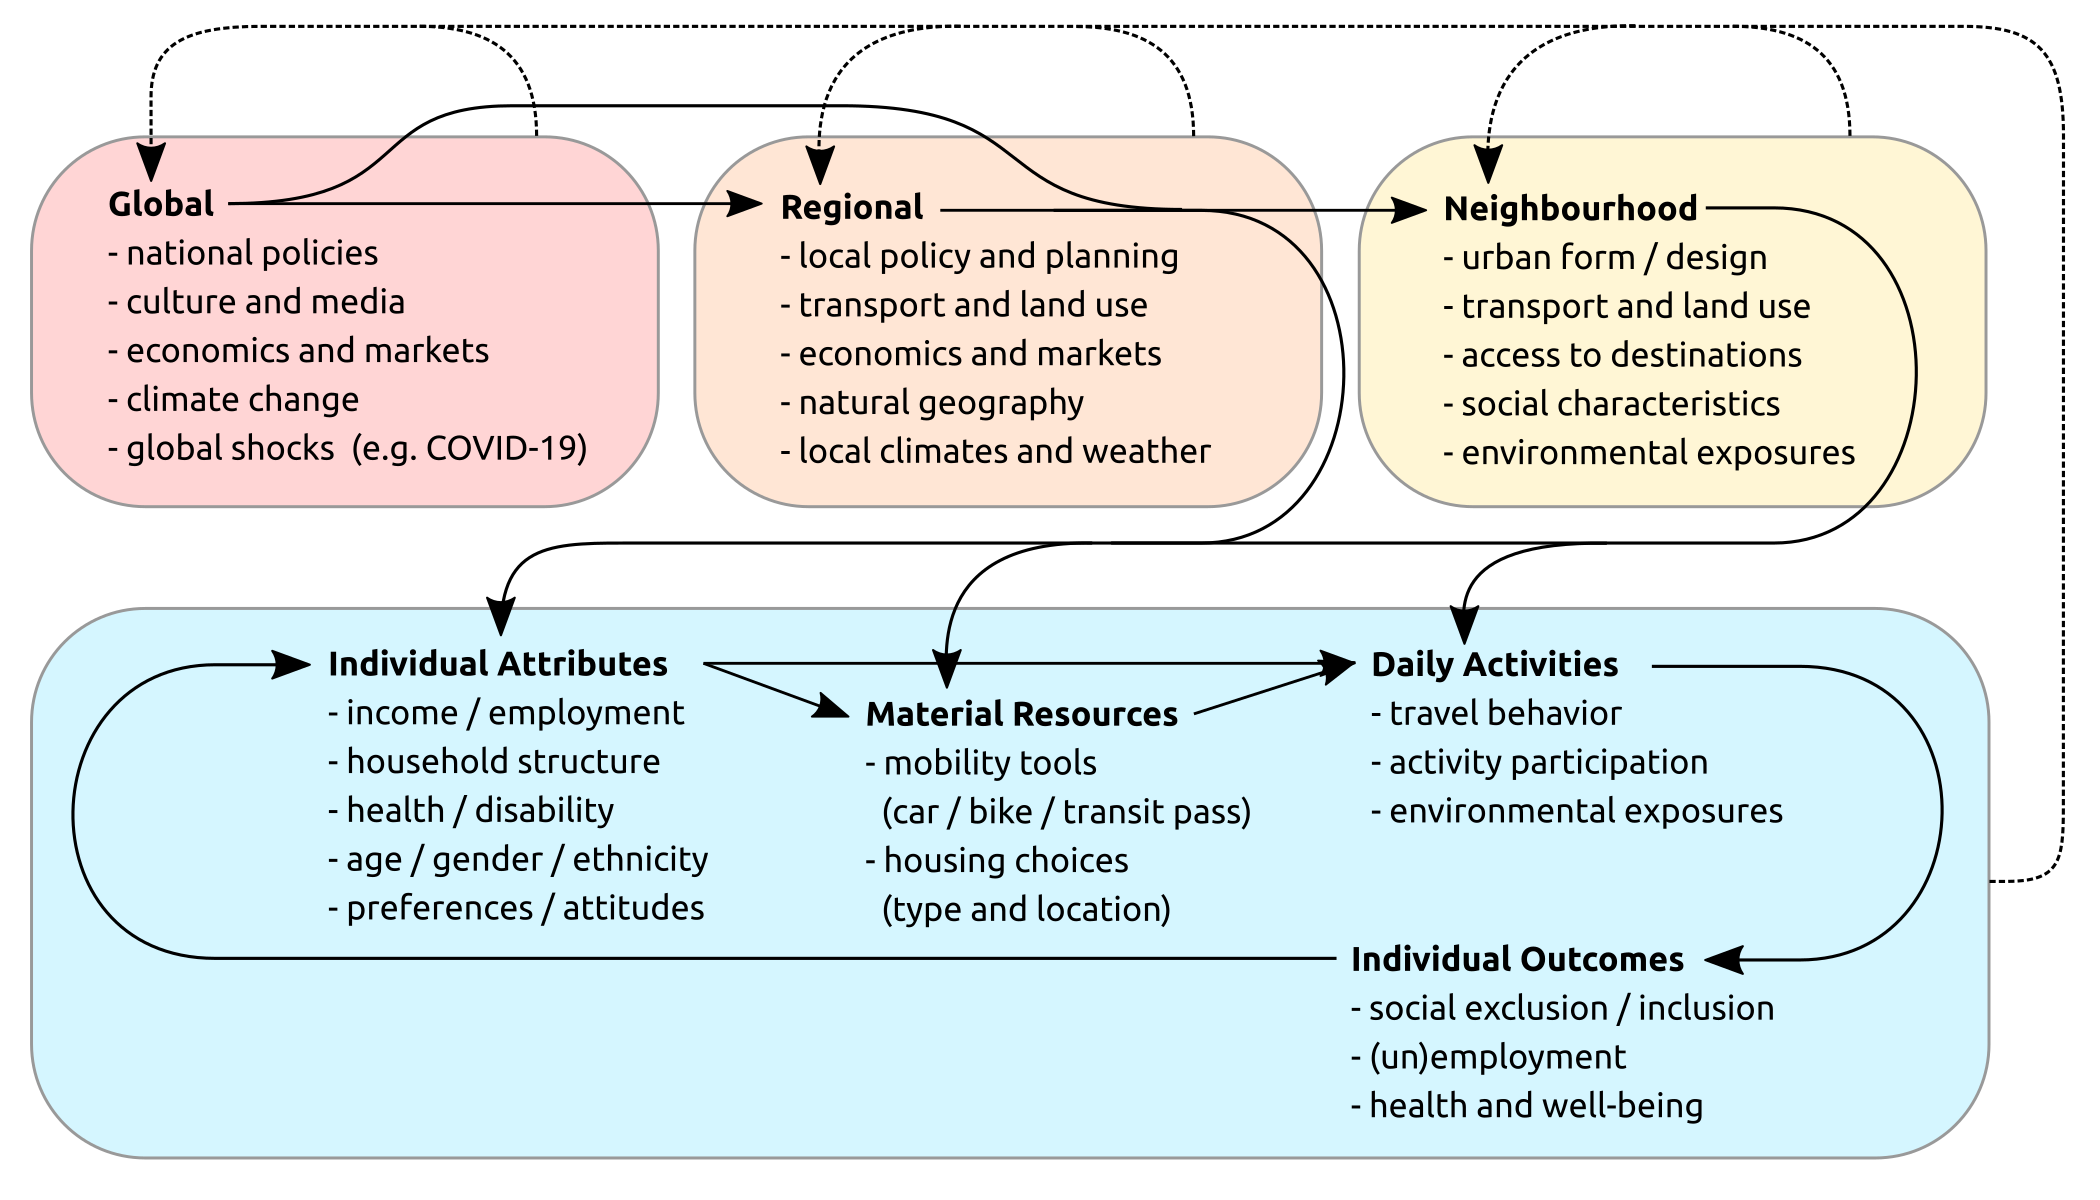
\includegraphics[width=6in]{figures/my_idea.png}
	\centering
	\label{fig:conceptual}
\end{figure}


Moreover, while the objective of our study was to examine changes across an entire region, another important direction for future work would be to map at a more localized scale whether there are neighbourhoods that have undergone high rates of out-mobility of low-income residents, and specifically if out-movers are decreasing their transit accessibility when moving, even if these trends are not prevalent at an aggregate regional level. This could provide more direct evidence into the locations within a region that are potentially experiencing residential displacement away from relied-upon public transit service.

Communication.



%
%In this section, we present a integrated conceptual framework to bring together the aforementioned conceptualizations of how geographic contexts effect individual outcomes, with how these geographic contexts can change over time. 
%
%Why is this important? Implications for research , while controlling , 
%
%human systems, urban systems, are complex - finding order within this complexity ...
%
%The overall framework is shown in Figure 2. This is divided into individual attributes and outcomes, geographic (i.e. neighbourhood) contexts, and global factors. The QQQ lines pertain to effects on individual choices and outcomes, while the QQQ lines pertain to aggregate effects of individuals on neighbourhood and regional characteristics.
%
%Sampson 2019/2012 - cogs micro/macro effects
%
%feedback - lucas
%
%UGCP - Kwan
%

% social outcomes, such as examining the impacts of changing environmental contexts on travel behaviour \cite{caoChangesNeighborhoodCharacteristics2007},









% transportation urban form income mobility - need data on auto ownership







%In particular, the Longitudinal Administrative Data/Databank/Database (LAD) will be the primary dataset for this paper, as it includes basic demographics (age, gender, marital status) and household structure (info about family members), as well as sources of income included in tax records. One limitation of this data, however, is it does not include information on car ownership, despite it being shown to be related to earnings in the long-term \cite{smart_disentangling_2020}.
%
%For methods, my current thinking is to model change in income, $\Delta I_i$ via a combination of level of accessibility, $A$, urban form, $U$, and controlling for demographic and households characteristics, $X$, and neighbourhood socio-economic variables, $N$.
%
%\[
%\Delta I_i = c + \alpha A_i + \mu U_i + \nu N_i + \beta X_i + \epsilon_i
%\]
%
%$\Delta I_i$ will be considered first as an absolute value pertaining to after-tax income, scaled to the most recent year's currency value. I will then convert income to measures of equivalent household income, which would then allow for generating measures of poverty based on the LIM methodology\footnote{divide income by the square root of households size, then compare with the distribution of all households. Those less than 50\% of the median are deemed to be under the poverty line}. 
%$N$, $A$, and $U$ will be based on one's average if they have moved to over the period of study. It will also be good to add a variable indicating residential mobility. The model will likely require incorporating multilevel effects, for both individual and neighbourhood scales. Spatial effects will be tested at the neighbourhood level. Another modelling option that I'll try to specify is more of an experimental design, where instead of a mean level of accessibility, $A$ and $U$ will be categorical variables pertaining to an increase, decrease, and no-change in accessibility for a specific time period, $t$, caused by a residential mobility event or opening of a new transit line. This strategy could be differentiated or combined for multiple intervention periods.
%
%Overall, the hope is that the sign and significance of the coefficients $\alpha$ and $\mu$ will offer evidence into whether, and to what extent, living in different types of built environments can have on income mobility and poverty reduction. Results will thus provide knowledge about whether and how the built environment (e.g. accessibility and urban form) can be a catalyst for neighbourhood SES change, and how different urban transport planning and design strategies can alleviate poverty.



% future transit accessibility

% Future forecasting with urban dynamics.





% \subsection{Communication}



